\documentclass{article} % For LaTeX2e
\usepackage{nips15submit_e,times}
\usepackage{hyperref}
\usepackage{url}
\usepackage[pdftex]{graphicx}
\usepackage{float}
\usepackage{amsmath}
\usepackage{amssymb}
%\documentstyle[nips14submit_09,times,art10]{article} % For LaTeX 2.09


\title{Information Retrieval and DataMining:\\
		Memory Models for Time Series Analysis
}


\author{
Mark Neumann, Alexander Chapovskiy and Zheng Tian\\ %thanks{} \\
UCL\\
\texttt{mark.neumann.15@ucl.ac.uk} \\
\texttt{alexander.chapovskiy.15@ucl.ac.uk} \\
\texttt{zheng.tian.11@ucl.ac.uk@ucl.ac.uk} \\
}
\newcommand{\fix}{\marginpar{FIX}}
\newcommand{\new}{\marginpar{NEW}}
\newcommand{\be}{\begin{equation}}
\newcommand{\ee}{\end{equation}}
\newcommand{\MSEtest}{MSE_{\rm \scriptsize test}}
%\DeclareMathOperator*{\tanh}{tanh}


\nipsfinalcopy % Uncomment for camera-ready version

\begin{document}


\maketitle
\graphicspath{{images/}}

\begin{abstract}
This is a report for group project in the Information Retrieval and Data 
Mining course. In this report we investigate different deep neural network
architectures on the time series. In particular, we apply neural 
networks to energy load and household energy consumption datasets.
\end{abstract}


\section{Introduction}
\label{sec:intro}

\subsection{Memory Models}
Long Short-Term memory\cite{LSTM} has been utilised widely across many disciplines in Machine Learning, with particularly notable performance in domains such as Machine Translation\cite{Sutskever}, Constituency Parsing\cite{Parsing}, Speech Recognition and even generative models, such as human level handwriting generation.\cite{Graves} 

Particularly key in the success of LSTM and other variants, such as the GRU, has been their perceived ability to selectively encode long-term dependencies and learn precise timings. In this work, we investigate the effect of precise timings in accurately modelling time-series data, an area which should particularly benefit from the accuracy features provided by Long Short-Term memory.

\subsection{Other Model Architectures}

One perceived failure of neural networks until recently was their inability to deal with arbitrary sequence lengths. The input dimensions to a standard LSTM classifier/regressor are fixed, meaning that data which intrinsically contains irreducible sequences of different lengths was difficult or impossible to process. This clearly is a problem with time series data, as the noisy nature of real world data means that we are rarely going to achieve perfectly timed and sanitised data.

In \cite{Sutskever}, Sutskever introduces sequence to sequence neural networks, which utilise two separate networks, one to encode a sentence into a vector representation and the other to decode a vector representation into the model ouptut. These are trained jointly, enabling arbitrary length sequences and particularly enabling non-monotonic transformations. We note that although we do not explore sequence to sequence models in this paper, the underlying cell structure we explore can be used in this architecture and that this is a very interesting area of development for time series models given their nature.  

\section{Datasets}
\label{sec:data}

\subsection{Energy Load}
\label{sec:data/energy}

!!!Description of the dataset

This dataset was used in the Kaggle competition. After the competition
the winners of the competition published their approaches, 
\cite{energy_kaggle}.
Mostly the approach is linear regression with non-linear features.

Neural networks are pplied to this dataset in \cite{enery_nn}

!!!! Before we apply out models to the dataset we perform the 
following preprocessing.\\

\subsection{Household Energy Consumption}
\label{sec:data/house}

\section{Regression with Non-linear Features}
\label{sec:reg}

In order to construct a baseline to examine our results, we performed linear regression with non-linear features on batches of one week's worth of data.
We use square root mean squared error divided by average load, achieving 12\% error using this metric. The figure below shows a representative week
for one of the zones with actual and predicted loads shown.

\begin{center}
\begin{tabular}{ccc}
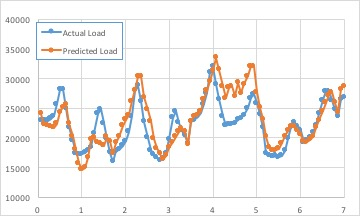
\includegraphics[width=0.6\linewidth]{LoadWeek.jpg} 
\end{tabular}
\end{center}



\section{Reccurent Neural Networks}
\label{sec:nn}

Below we describe the models applied to the dataset, for which performance can be found in the next section. In addition to vanilla Long Short-Term Memory, we explore several recent innovations over the last few years, including Gated Recurrent Units and peephole connections. 



\subsection{LSTM}
\label{sec:nn/lstm}


Given an input vector $x_{t} \in \mathbb{R}^{N}$ at time $t$ and the previous output of the LSTM $h_{t-1} \in \mathbb{R}^{K}$, the forget gate($f_{t}$), the input gate($i_{t}$), the output gate($o_{t}$) and the cell input($z_{t}$) are computed as follows:
\begin{equation}
\begin{aligned}[c]
    H &= \left[ \begin{array}{cc}
         x_{t}  \\
         h_{t-1} 
    \end{array} \right] \in \mathbb{R}^{N+K} \\
    z_{t} &= Tanh(W_{z}H + b_{z}) \\
    i_{t} &= \sigma(W_{i}H + b_{i})\\
    \end{aligned}
    \qquad \qquad
    \begin{aligned}[c]
    o_{t} &= \sigma(W_{o}H + b_{o})\\
    f_{t} &= \sigma(W_{i}H + b_{i})\\
    c_{t} &= f_{t} \odot c_{t-1} + i_{t} \odot z_{t} \\
    h_{t} &= o_{t} \odot Tanh(c_{t}) \\
    \end{aligned}
\end{equation}

Where $W_{z}, W_{i}, W_{o}, W_{f} \in \mathbb{R}^{K \times(N+K)}$ and $b_{z}, b_{i}, b_{o}, b_{f} \in \mathbb{R}^{K}$ are trained weight matrices and bias vectors for $N$, the dimension of the input vector and $K$ the hidden size of the LSTM. $\sigma$ and $Tanh$ are element-wise activation functions representing the sigmoid and hyperbolic tangent functions, with $\odot$ representing element-wise multiplication. 

Below we present a pictorial demonstration of the connections in the LSTM cell. 

\begin{figure}[H]
\begin{center}

\includegraphics[width=0.8 \linewidth]{LSTM.png} 
\end{center}
\caption{A demonstration of the interactions within an LSTM cell. Here we can see clearly how the input and output control the respective features of the cell: the closer to zero these vectors are, the smaller the amount of information which can travel through the dot product.}
\end{figure}




\subsection{Gated Recurrent Unit}
\label{sec:nn/gru}

The Gated Recurrent Unit\cite{DBLP:journals/corr/ChungGCB15} can be seen as a simplified LSTM with a tied output and forget gate, merging two of the above equations. 

Given an input vector $x_{t} \in \mathbb{R}^{N}$ at time $t$ and the previous output of the GRU $h_{t-1} \in \mathbb{R}^{K}$, the forget gate($f_{t}$), the input gate($i_{t}$) and cell output($h_{t}$)  are computed as follows:
\begin{equation}
\begin{aligned}[c]
         &Input: x_{t}  \\
         &Prev State: h_{t-1} \\
    	 &i_{t} = \sigma(W_{i}^{x}x_{t} + W_{i}^{h} h_{t-1} + b_{i})\\
    \end{aligned}
    \qquad \qquad
    \begin{aligned}[c]
    f_{t} &= \sigma(W_{f}^{x}x_{t} + W_{f}^{h} h_{t-1} + b_{f})\\
    \tilde{h_{t}} &= Tanh(W x_{t} + f_{t} \odot h_{t-1})\\
    h_{t} &= i_{t} \odot h_{t-1} + (1- z_{t}) \odot \tilde{h_t}  \\
    \end{aligned}
\end{equation}

Where $W_{i}^{x}, W_{f}^{x}, \in \mathbb{R}^{K \times(N)}, W_{i}^{h}, W_{f}^{h} \in \mathbb{R}^{K \times(K)}$ and $b_{i} \in \mathbb{R}^{N}, b_{f} \in \mathbb{R}^{K}$ are trained weight matrices and bias vectors for $N$, the dimension of the input vector and $K$ the hidden size of the GRU. $\sigma$ and $Tanh$ are again element-wise activation functions representing the sigmoid and hyperbolic tangent functions, with $\odot$ representing element-wise multiplication as above. 

It should be noted that subsequent papers by Cho expand on the GRU, particularly to incorporate "recurrent feedback", intuitively described as a linear combination of memory storage across hidden layers. This would certainly be an interesting extension to the work in this paper.


\subsection{Peephole Connections}
\label{sec:nn/peephole}

Peephole connections are a popular addition to the Long Short-Term memory model\cite{peepholeconnections}. Originating in a paper by Schmidhuber and Gers whilst working at the IDSIA lab in Switzerland, they quickly became popular in an array of literature. The basic premise is that the gates of the LSTM mechanism become a function not only of the current input $x_{t}$ and previous LSTM state $h_{h-1}$, but also a function of the current cell memory state which persists from the last timestep,  $c_{t-1}$. The input, output and forget gates are therefore defined as follows:

\begin{equation}
\begin{aligned}[c]
 H &= \left[ \begin{array}{cc}
         x_{t}  \\
         h_{t-1} \\
         c_{t-1}
    \end{array} \right] \in \mathbb{R}^{N+2K} \\
\end{aligned}
\qquad \qquad
    \begin{aligned}[c]
    i_{t} &= \sigma(W_{i}H + b_{i})\\
    f_{t} &= \sigma(W_{f}H + b_{f})\\
    o_{t} &= \sigma(W_{o}^{x}x_{t} + W_{o}^{h}h_{t-1} + W_{o}^{c}c_{t} +  + b_{o})\\
    \end{aligned}
\end{equation}

where the memory is simply appended onto the vector used in the LSTM mechanism for the calculation of the input and forget gates, with the output gate using a different format only because it uses the {\it current} state's memory, rather than the previous one as in the input and forget gates. The other functionality remains unchanged. Additionally, some practitioners choose to only apply peephole connections to gates selectively - often, they are only applied to the input and output gates and not the forget gate. Note the effect of peephole connections is difficult to measure accurately, as in a vanilla LSTM, all the gates are implicitly a function of the memory vector, as they are a function of the previous state which is informed by the memory at that point. Below we present a pictorial representation of how the addition of peephole connections changes the internal cell architecture.

\begin{figure}[H]
\begin{center}
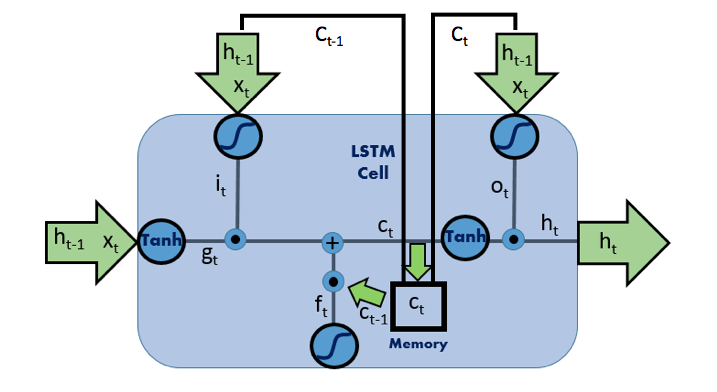
\includegraphics[width=0.8 \linewidth]{LSTM_Peepholes.png} 
\end{center}
\caption{Here we can clearly see how all gates now have direct interaction with the memory state.}
\end{figure}



\section{Results}
\label{sec:nn/results}



\section{Conclusions}

Overall, we have examined the performance of peephole connections and neural network architectures in general for several tasks, drawing mixed results. 




\begin{thebibliography}{9}


\small{


\bibitem{energy_kaggle}
Tao Hong, Pierre Pinson and Shu Fan, 
(2014), {\it Global Energy Forecasting Competition 2012.}
International Journal of Forecasting, 30(2), 357;
\\

\bibitem{DBLP:journals/corr/ChungGCB15}

Junyoung Chung and
               {\c{C}}aglar G{\"{u}}l{\c{c}}ehre and
               KyungHyun Cho and
               Yoshua Bengio (2014)
{\it Gated Recurrent Neural Networks}

\bibitem{peepholeconnections}

Gers, F. and Schmidhuber, J. (2000)
{\it  Recurrent Nets that time and Count} 

\bibitem{Sutskever}

Sutskever, I., Vinyals, O., Le, Q.V. (2015)

{\it Sequence to Sequence Learning with Neural Networks}


\bibitem{Graves}
Graves, A. (2013)
{\it Generating Sequences With Recurrent Neural Networks}

\bibitem{Parsing}
Oriol Vinyals and
               Lukasz Kaiser and
               Terry Koo and
               Slav Petrov and
               Ilya Sutskever and
               Geoffrey E. Hinton, (2015)
\it{Grammar as a Foreign Language}

\bibitem{LSTM}

Sepp Hochreiter and J�rgen Schmidhuber(1995)
{\it Long Short-Term Memory}

Charlton, N. and Singleton, C. 
(2014). 
{\it A refined parametric model for short term load forecasting.}
International Journal of Forecasting,
30(2), 364-368.
\\
Souhaib Ben Taieba and Rob J. Hyndmanb,
(2014), 
{\it A gradient boosting approach to the Kaggle load forecasting 
competition.}
International Journal of Forecasting, 30(2), 382;
\\
Lloyd, J. R. (2014), 
{\it GEFCom2012 hierarchical load forecasting: Gradient boosting machines and Gaussian processes. }
International Journal of Forecasting, 30(2), 369.


}

\end{thebibliography}

\end{document}
